\documentclass{article}
\usepackage{graphicx}
\usepackage{float}
\usepackage{subcaption}
\usepackage{amsmath}
\usepackage[colorlinks=true, allcolors=blue]{hyperref}

\bibliographystyle{alpha}

\title{Information Theory \\ \large Problem set 02 - Probability, entropy and inference}
\author{Luís Felipe Ramos Ferreira}
\date{\href{mailto:lframos\_ferreira@outlook.com}{\texttt{lframos\_ferreira@outlook.com}}
}

\begin{document}

\maketitle

\begin{enumerate}
    \item \begin{enumerate}
            \item The frequentist interpretation of probability is, obviously, associated with the concept of frequency. It states that the probability \(p(s)\) of a event \(s\) should reflect the frequency that the event \(s\) happens compared to the rest of the events in the sample space, as the number of experiments goes to infinity. On the other hand, the bayesian interpretation of probability is more subjective, as it assumes the probability \(p(s)\) of a event \(s\) is the degree of belief we should have that the outcome of an experiment in the sample space will be \(s\).
            \item b
            \item c
    \end{enumerate}

    \item Obviously, the probability that the first ball is white, \(P_f\), is equal to \(\frac{w}{w + b}\), since there are \(w + b\) balls and \(w\) of them are white. Let's calculate now the event of the second ball being white. We should consider that the first ball can be either white or black in this case, and each outcome for the first ball can affect the outcome for the second ball. So, we have that the probability \(P_s\) of the second ball being white is defined as the sum of the probability that the second ball is white given the fact the first ball was white and the probability that the second ball is white given that the first ball was black. In mathematical terms, it would be:
    \begin{gather}
        P_s = P_f\frac{w - 1}{w - 1 + b} + (1 - P_f)\frac{w}{w + b - 1} \\
        P_s = P_f\frac{w}{w + b - 1} - \frac{P_f}{w + b - 1} + \frac{w}{w + b - 1} - P_f\frac{w}{w + b - 1} \\
        P_s = \frac{w - P_f}{w + b - 1} \\
        P_s = \frac{w - \frac{w}{w + b}}{w + b - 1} \\
        P_s = \frac{w(w + b) - w}{(w + b - 1)(w + b)} \\
        P_s = \frac{w(w + b - 1)}{(w + b - 1)(w + b)} \\
        P_s = \frac{w}{w + b} 
    \end{gather}

    At the end, we have what we expected, \(P_f = P_s = \frac{w}{w + b}\).

    \item Question answered by hand
	\begin{figure}[H]
		\centering
		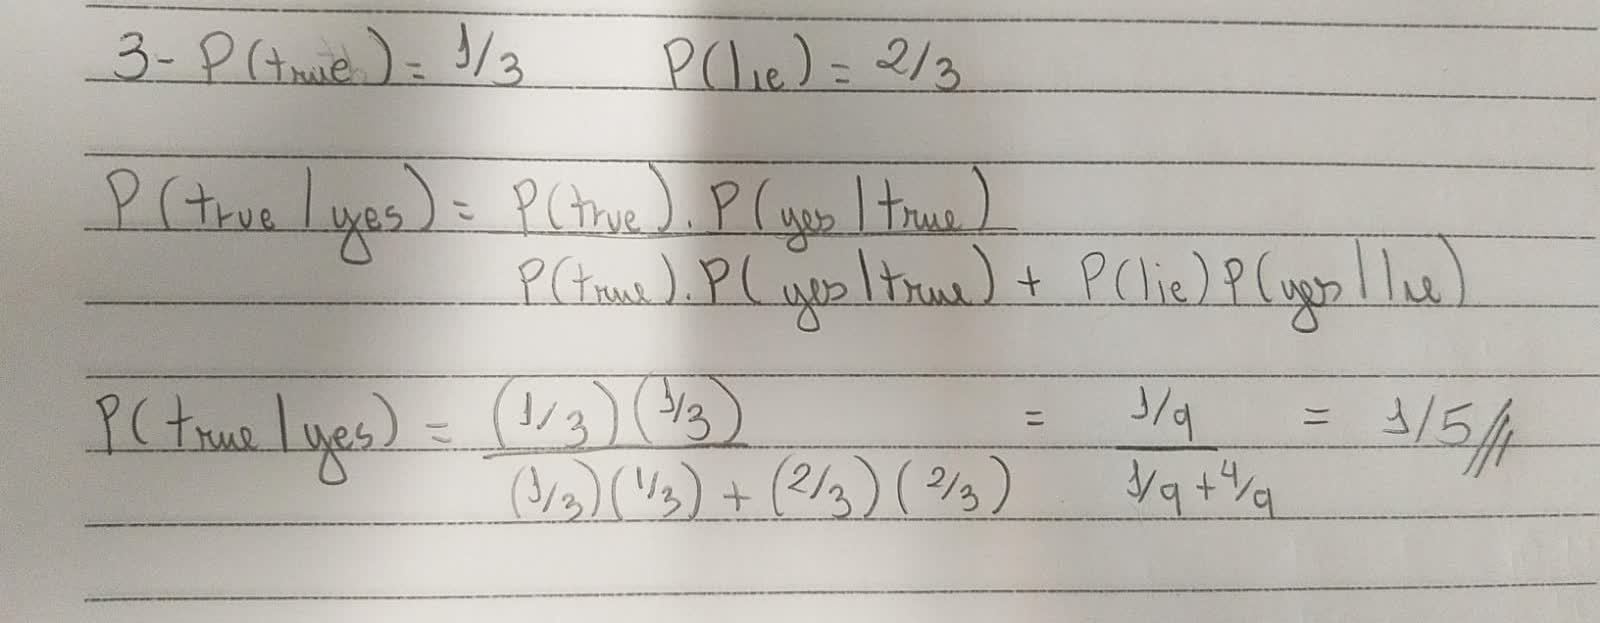
\includegraphics[width=0.5\textwidth]{images/03.jpeg}
		\caption{Problem 03}
	\end{figure}

\item No, the lawyer is wrong and is either ignorant about probability or a slimy trickster. Althought what he said is true, that is, the probability that Mrs S was murdered by her husband, given the fact he used to beat her, is \(\frac{1}{1000}\), there is data not added to the argument.
NOT ANSWERED YET

\item There are three posible states of the experiment that should be considered:
	\begin{itemize}
		\item The original counter was black and we removed the white counter that was added afterwards
		\item The original counter was white and we removed the white counter that was added afterwards
		\item The original counter was white and we removed the original counter
	\end{itemize}
		Note that there are 3 posible outcomes in the sample space, but only 2 of them have the remaining counter in the bag of the color white. Therefore, the answer to the question is \(\frac{2}{3}\).
\end{enumerate}

\end{document}
